\section{Burndown Charts}
The team put effort into trying to estimate every task they added and worked on during the project.\\
This enabled Visual Studio Online to create graphical burndown charts of the work completed. These provided a nice overview of how the sprint had gone at every retrospection.

\subsection{Sprint 1}
The burndown chart after sprint one reflects how the team stayed within their limits. \\
Team members were not assigned a extrordinary amount of tasks and they completed the tasks within the set time frame.

\begin{figure}[H]
	\centering
	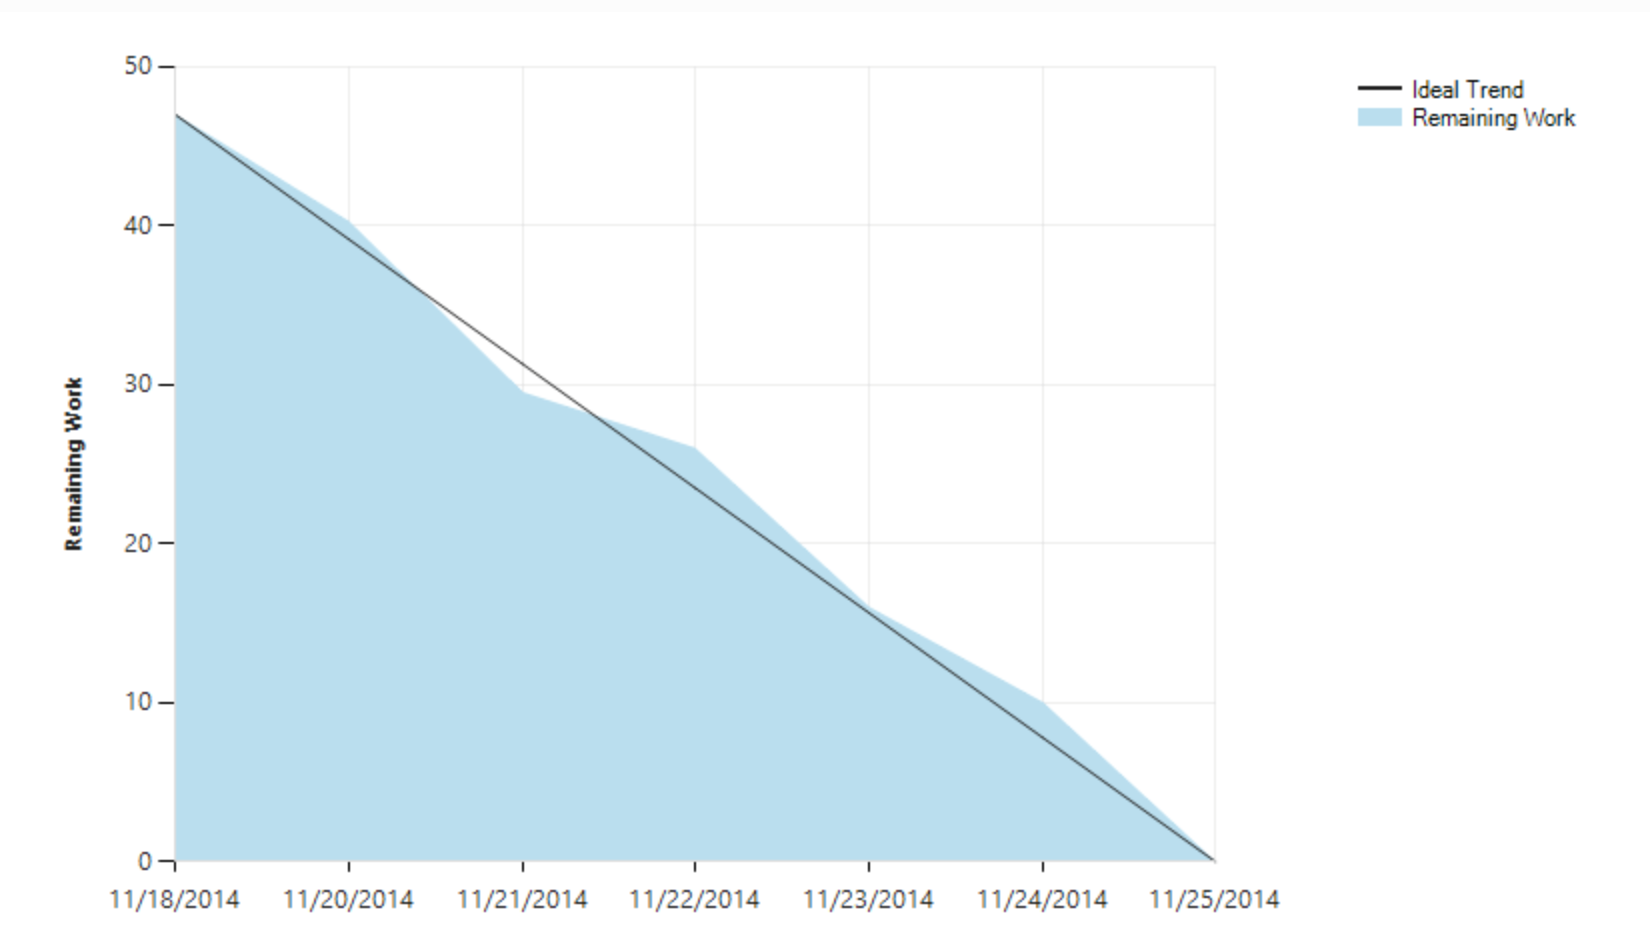
\includegraphics[scale=0.40]{Figures/Burndown1}
	% place the figure in the Figures folder (located with the main file)
	% you need to fix the scale a few times to get it right, but latex does not compress so one can always zoom in to see details.
	\caption{Burndown Chart after Sprint 1.}
\end{figure}

\subsection{Sprint 2}
The burndown chart after sprint two reflects how the team changed tactics. \\
It was decided at the sprint planning meeting after sprint one to have an aggressive amount of work assigned to every team member, in order to complete a larger amount of work. \\
Team members discussed not being able to complete \textit{every} task and focus on having a working prototype ready for the end of the sprint.\\
Note the total amount of hours at the top of the chart and the hump near the end. Also note that the team did not complete every assignment, but got the main tasks out of the way.

\begin{figure}[H]
	\centering
	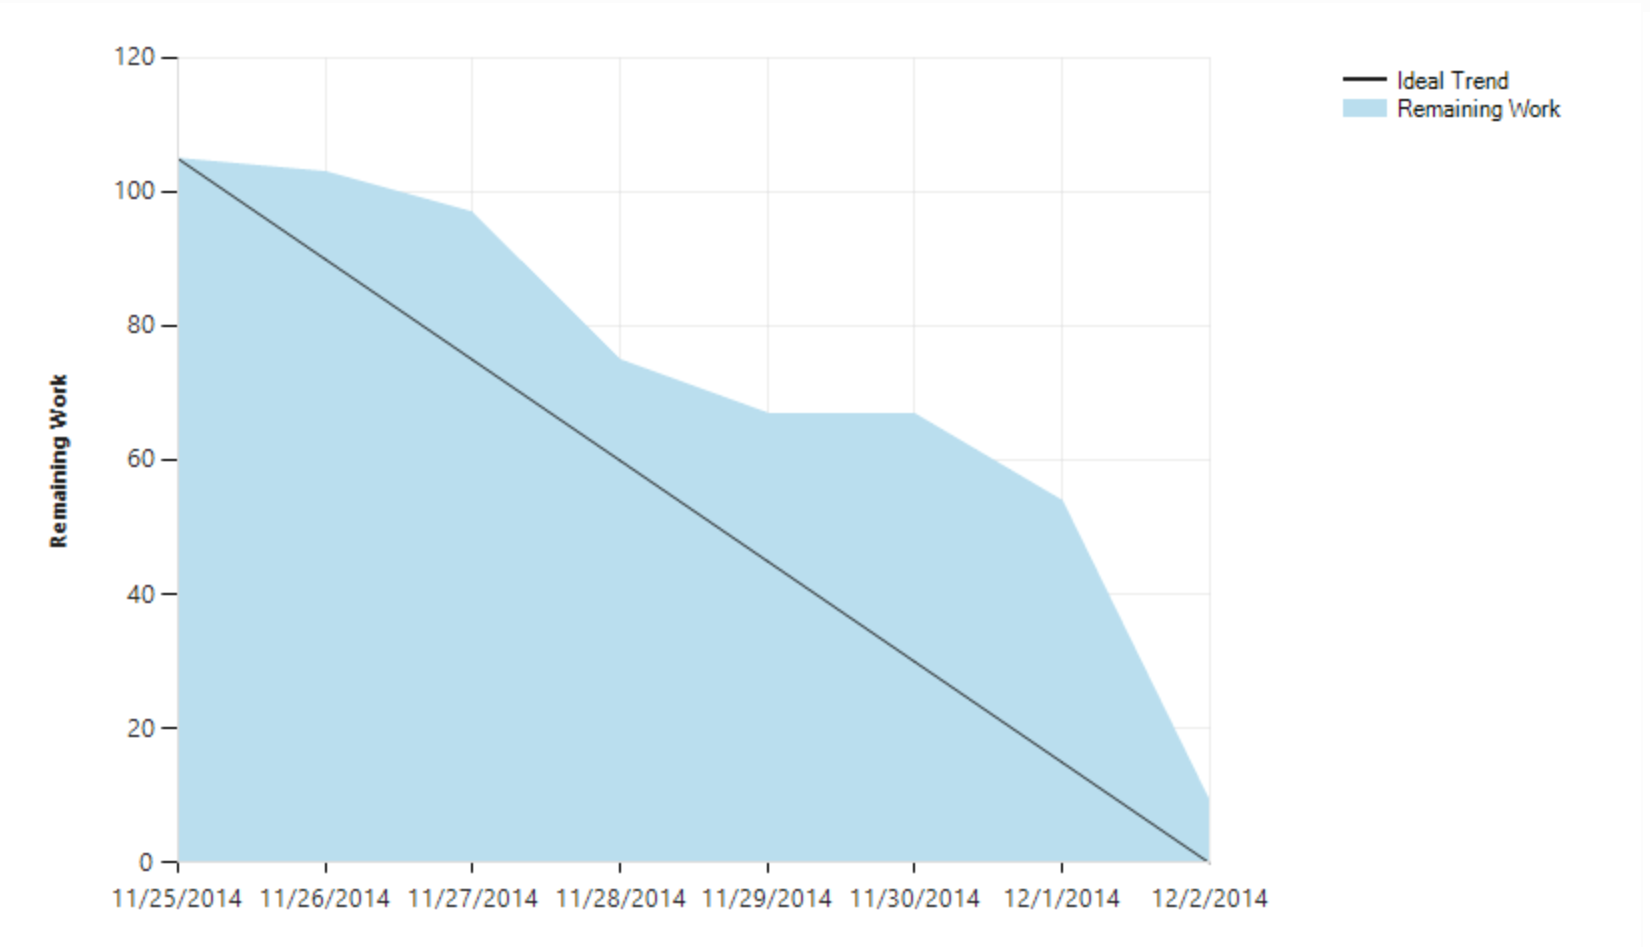
\includegraphics[scale=0.40]{Figures/Burndown2}
	% place the figure in the Figures folder (located with the main file)
	% you need to fix the scale a few times to get it right, but latex does not compress so one can always zoom in to see details.
	\caption{Burndown Chart after Sprint 2.}
\end{figure}

\subsection{Sprint 3}
The burndown chart after sprint three reflects how the team found a reasonable amount of work. \\
After having finished a working prototype the workload returned to a more "relaxed" amount.

\begin{figure}[H]
	\centering
	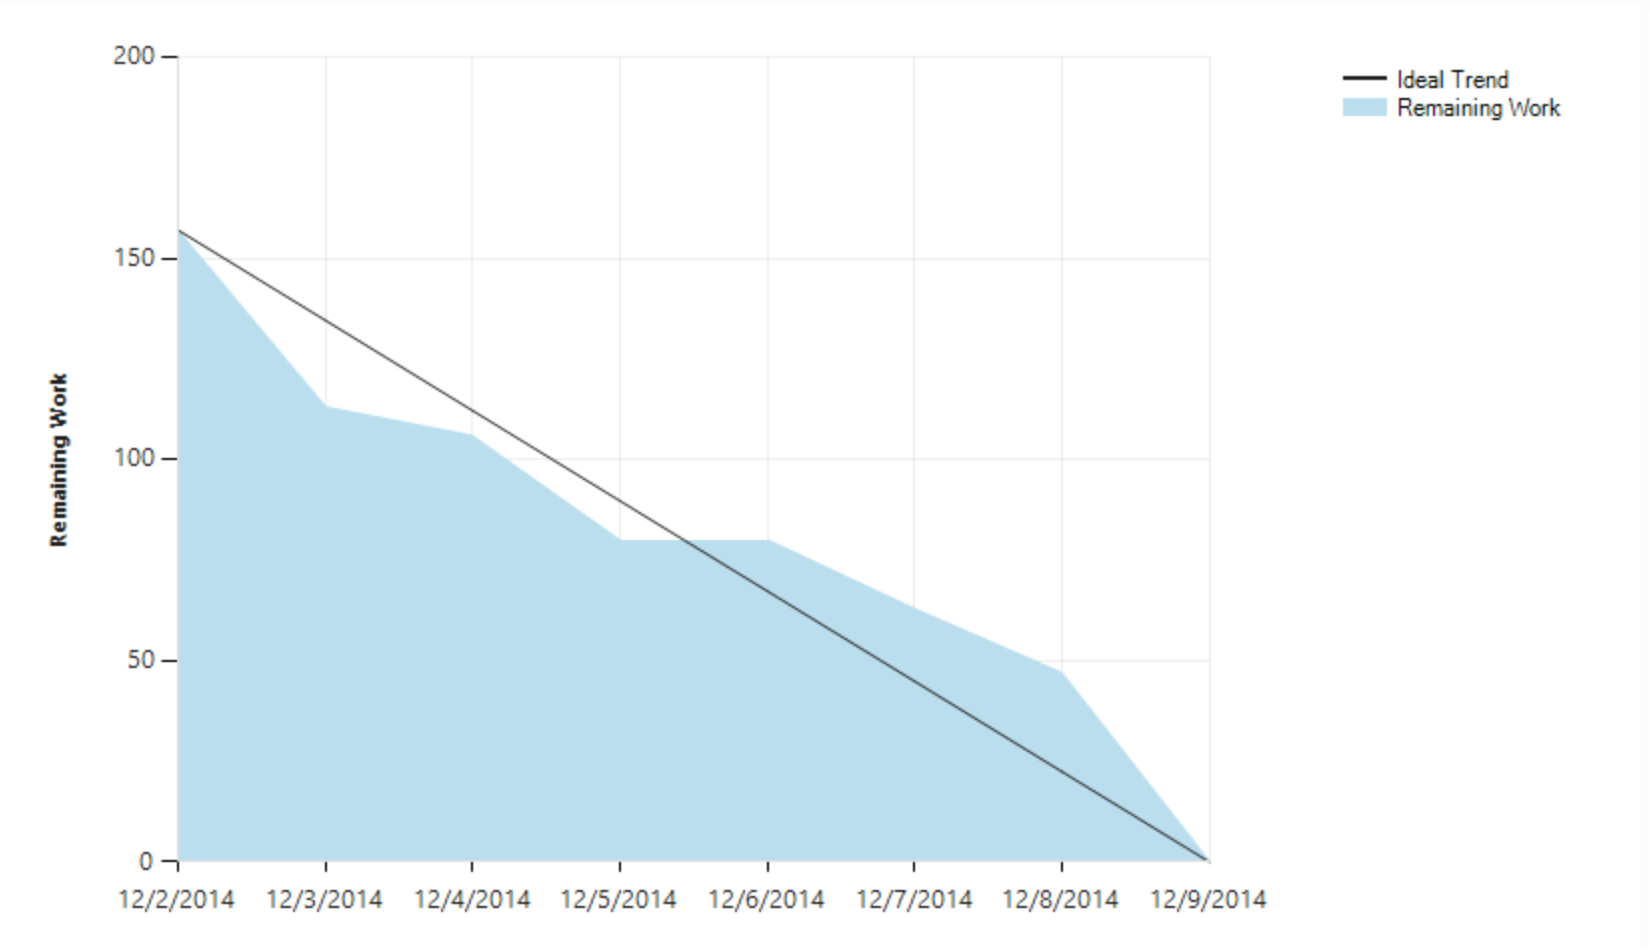
\includegraphics[scale=0.40]{Figures/Burndown3}
	% place the figure in the Figures folder (located with the main file)
	% you need to fix the scale a few times to get it right, but latex does not compress so one can always zoom in to see details.
	\caption{Burndown Chart after Sprint 3.}
\end{figure}

\subsection{Sprint 4}
The burndown chart after sprint four reflects how the team didn't use the online SCRUM tool and instead worked on items they felt needed work to be finished. The burndown chart reflects this in that it does not follow the expected graph. All work was finished, but sometimes not put into the system.\todo{change the figure} \\

\begin{figure}[H]
	\centering
	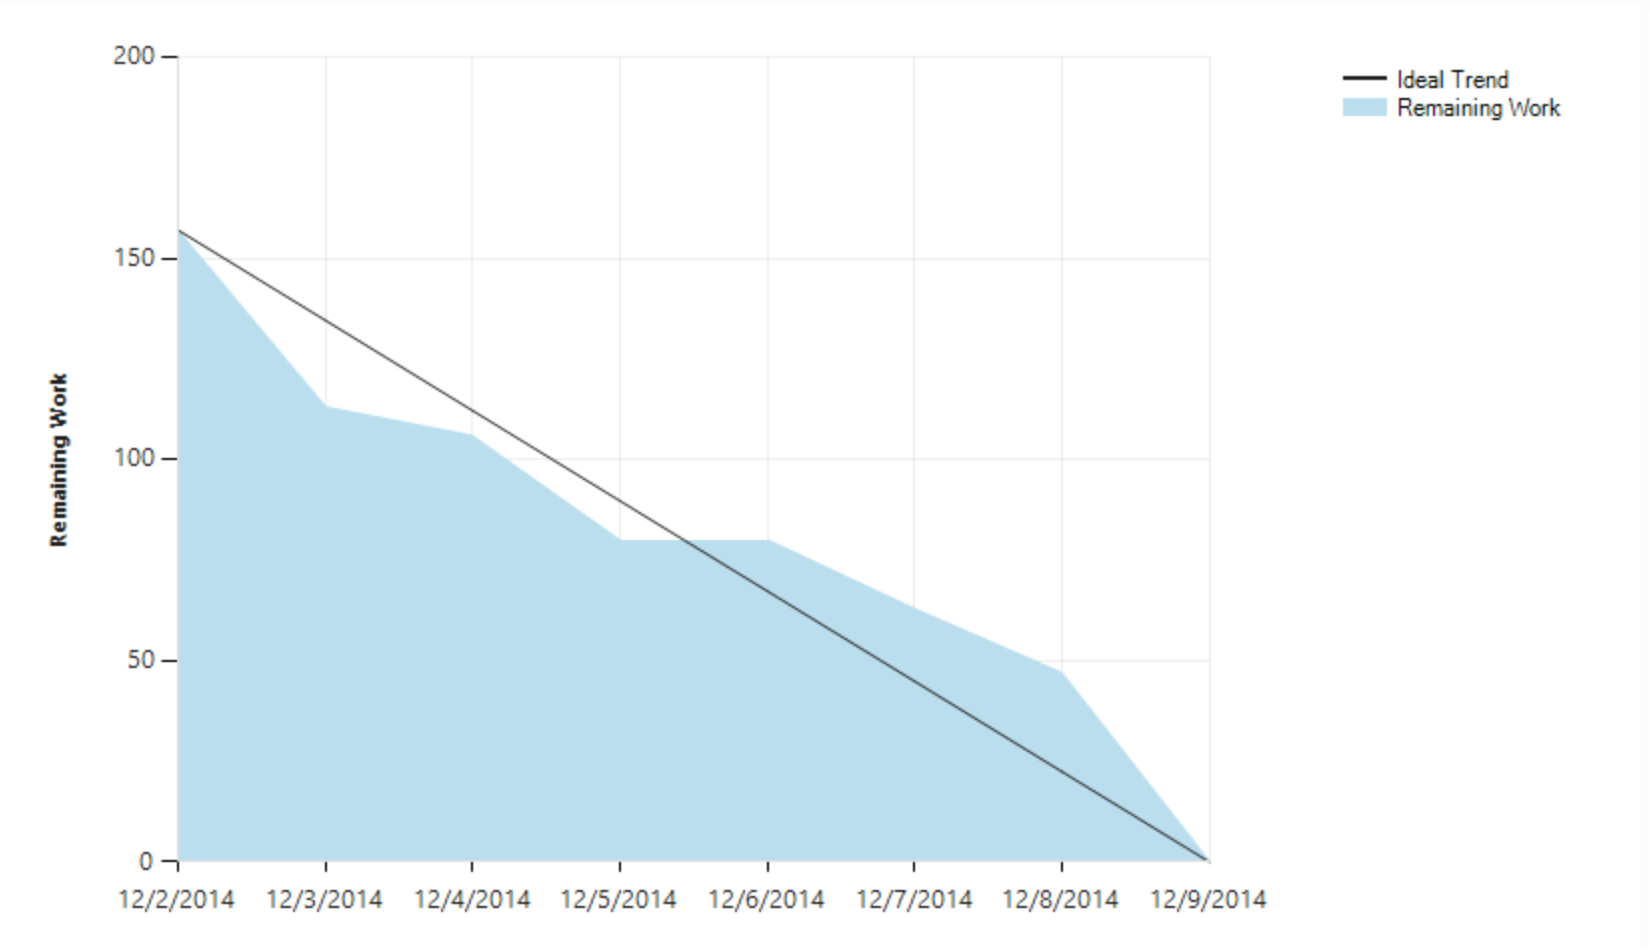
\includegraphics[scale=0.40]{Figures/Burndown3}
	% place the figure in the Figures folder (located with the main file)
	% you need to fix the scale a few times to get it right, but latex does not compress so one can always zoom in to see details.
	\caption{Burndown Chart after Sprint 4.}
\end{figure}